\chapter{ProgBot - Um Assistente Especialista em Programação Orientada a Objetos}

\begin{flushright}
Luis Paulo da Silva Carvalho
\end{flushright}

ProgBot é um Assistente Virtual Especialista em Programação Orientada a Objetos (POO). O objetivo dele é prestar auxílio a usuários que desejam saber mais sobre tal técnica de programação e sobre como melhorar os códigos-fonte de seus programas.

Mesmo com a atual evolução da Inteligência Artificial (IA) e seu uso durante o desenvolvimento de Sistemas de Informação (SI) \cite{yamada2026impactos}, ainda existe a necessidade de aprofundamento, seja no ambiente acadêmico e até mesmo na indústria de software, o que impõe desafios ao efetivo ensino de POO \cite{sperotto2025metodologias}. 

O desenvolvimento do ProgBot buscou a união entre IA e a atividade de aprendizado de POO. A solução utiliza modelos de IA, contextualizados via criação de personas virtuais (\textit{prompts}), para disponibilizar uma experiência de conversaçãl (\textit{chat}) para usuários interessados em desenvolvimento de SIs.

As seções seguintes fornecem detalhes sobre o processo de desenvolvimento e os principais componentes e módulos integrados e criados para tornar o ProgBot operacional.

\section{Arquitetura do ProgBot}

A Figura \ref{fig:arquitetura-progbot} exibe a arquitetura de interfaces e componentes do ProgBot. O usuário se comunica com o núcleo do SE através de uma sala de chat. O chat envia a mensagem ou pergunta para o núcleo onde um LLM, inicialmente configurado por um \textit{prompt} para assumir um papel ou persona, processa a pergunta através de sua rede neural, que funciona como um motor de inferência. O LLM é configurado para responder as perguntas especificadas na base de conhecimento também através de {prompt}, devendo se abster de perguntas que não estejam relacionadas com POO. A memória de trabalho é mantida através da combinação de dois componentes: (i) um cache semântico, que consegue recuperar, por similaridade, a resposta para perguntas (semanticamente) similar a perguntas anteriores, e (ii) a adição de toda a pilha de mensagens trocadas entre o usuário e o LLM ao contexto de acesso à API do Gemini.

\begin{figure}[htbp]
\centering
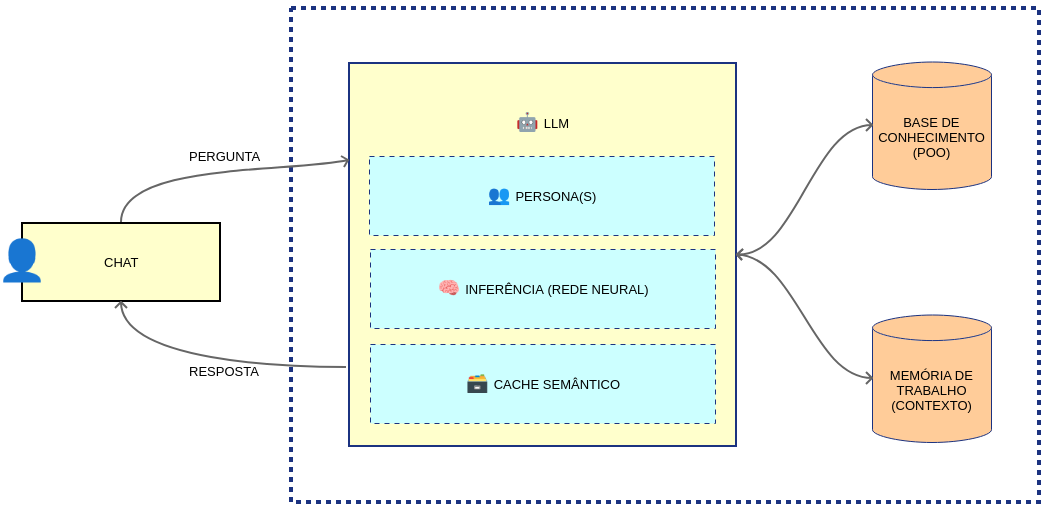
\includegraphics[width=1.0\textwidth]{capitulos/capitulo_1/arquitetura.png}
\caption{Arquitetura do ProgBot}
\label{fig:arquitetura-progbot}
\end{figure}

\section{Ferramentas MCP}

Quando uma aplicação com LLM se conecta a ferramentas por meio do MCP, o protocolo oferece uma interface padronizada para descobrir e invocar capacidades externas e incorporar os resultados ao fluxo de interação \cite{mcp2026architecture}. Assim, o sistema pode complementar a geração de texto com ações executadas por serviços especializados. No ProgBot, isso permite combinar as respostas do modelo com verificações de linguagem de programação e sintaxe, oferecendo retorno mais contextualizado e prático ao usuário.

O ProgBot disponibiliza duas ferramentas: \path{detectar_linguagem}, que identifica a linguagem de programação utilizada em um trecho de código, evitando que o usuário precise informá-la manualmente; e \path{verificar_sintaxe}, que confere se o código segue as regras sintáticas da linguagem indicada e aponta quando há erros. Em conjunto, elas facilitam a análise inicial do código e ajudam o usuário a localizar problemas de sintaxe.

\section{Desenvolvimento e Avaliação}

O ProgBot foi desenvolvido em Python, integrando bibliotecas com funções complementares. A \textit{sentence-transformers} converte perguntas e trechos da base de conhecimento em \textit{embeddings}, que possibilitam comparar a similaridade entre a consulta e os conteúdos. O \textit{chromadb} armazena vetores de representação numérica dos \textit{embeddings}. A biblioteca, \textit{google-genai}, permite enviar instruções e contexto à API do Gemini e receber a resposta gerada. O \texttt{FastMCP} é usado para disponibilizar ferramentas e recursos por meio do protocolo MCP. Desse modo, conteúdos recuperados podem ser fornecidos ao modelo como contexto adicional para processamento de código-fonte. 

O resultado da união desses recursos pode ser visto na Figura \ref{fig:funcionamento-progbot}. É possível visualizar a interação do usuário com o ProgBot e também a possibilidade de uso das ferramentas MCP.

\begin{figure}[htbp]
\centering
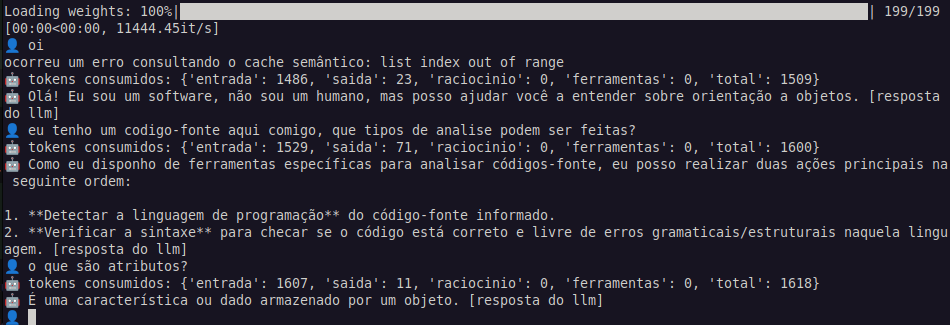
\includegraphics[width=1.0\textwidth]{capitulos/capitulo_1/funcionamento.png}
\caption{Funcionamento do ProgBot}
\label{fig:funcionamento-progbot}
\end{figure}

Para testar a qualidade das respostas, aplica-se a técnica \textit{LLM-as-a-Judge}. Para cada pergunta de avaliação, um julgador analisa a pergunta e a resposta do ProgBot. Respostas que não são consideradas adequadas podem ser usadas para identificar ajustes necessários nos \textit{prompts} ou na escolha dos LLMs utilizados para realizar as inferências sobre as perguntas do usuários. O resultado do julgamento pode ser visto na Figura \ref{fig:julgamento-progbot}.

\begin{figure}[htbp]
\centering
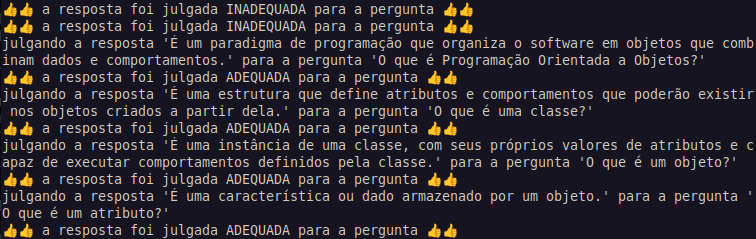
\includegraphics[width=1.0\textwidth]{capitulos/capitulo_1/julgamento.png}
\caption{Julgamento do ProgBot}
\label{fig:julgamento-progbot}
\end{figure}

\section{Reproducibilidade e Reuso}

O código-fonte do ProgBot pode ser consultado e (re)usado livremente através do link de acesso ao \href{https://zenodo.org/records/23445337?preview_file=progbot.zip}{repositório do projeto}. Também se encontra disponibilizado um vídeo demonstrativo \href{https://zenodo.org/records/23428906/preview/progbot.mp4}{neste link}. 